
\section{Perfilado de código}

El perfilado de código (\textit{profiling}) es el proceso de medir el comportamiento
de un programa en ejecución con el objetivo de identificar dónde se concentra el
costo computacional y de memoria.
A diferencia del análisis estático, el perfilado opera sobre la ejecución real del
programa, capturando métricas como tiempo por función, contadores de hardware del
procesador, comportamiento de la jerarquía de caché y consumo dinámico de memoria.
Esto permite construir evidencia empírica que justifica las decisiones de optimización
y sirve de línea base para comparar implementaciones alternativas.

El script \texttt{bench\_profiling.sh} orquesta cinco técnicas de perfilado
complementarias sobre la implementación secuencial del autómata celular de tráfico,
para los tamaños de carretera $N \in \{8000, 64000, 500000, 2000000\}$ con densidad
fija de 0.50 y 1000 pasos de simulación por medición.
Cada técnica responde una pregunta distinta: cuánto tiempo tarda, en qué función
se acumula ese tiempo, qué eventos de hardware ocurren, qué nivel de caché sirve
los accesos, y cuánta memoria dinámica se consume.
Los resultados se consolidan en un archivo CSV (\texttt{data\_profiling.csv}) que
sirve de entrada al generador de reportes.


\subsection{Binarios compilados}

El script genera dos binarios distintos a partir de las mismas fuentes
(\texttt{road.c}, \texttt{simulation.c}, \texttt{cli\_args.c}, \texttt{timing.c},
\texttt{seq\_main.c}):

\begin{itemize}
    \item El binario \texttt{traffic\_seq\_perf} se compila con
        \texttt{gcc -g -std=c11 -D\_POSIX\_C\_SOURCE=200809L}, sin optimizaciones
        de nivel, activando símbolos de depuración (\texttt{-g}) para que perf y
        Valgrind puedan asociar las muestras con el código fuente.
        Este binario es el que utilizan perf stat, perf record, Valgrind Massif y
        Valgrind Cachegrind.

    \item El binario \texttt{traffic\_seq\_gprof} se compila adicionalmente con
        \texttt{-fno-inline -pg}.
        La flag \texttt{-pg} instruye al compilador para insertar llamadas a
        \texttt{mcount()} al inicio de cada función, generando el archivo
        \texttt{gmon.out} durante la ejecución.
        La flag \texttt{-fno-inline} impide que el compilador funda el cuerpo de
        funciones pequeñas en sus sitios de llamada, garantizando que gprof pueda
        contabilizar cada función de forma independiente.
\end{itemize}


\subsection{gprof: perfilado por instrumentación del compilador}

\texttt{gprof} es una herramienta de perfilado basada en instrumentación generada
en tiempo de compilación.
El script ejecuta \texttt{traffic\_seq\_gprof} con los mismos parámetros de
calentamiento y medición, lo que genera el archivo \texttt{gmon.out}, y luego
invoca \texttt{gprof} para producir el reporte textual.

El reporte tiene dos partes principales.
El \textit{flat profile} lista cada función con el porcentaje del tiempo total que
le corresponde, los segundos acumulados, el número de invocaciones y el tiempo
promedio por llamada; responde directamente la pregunta de en qué función pasa el
programa la mayor parte del tiempo.
El \textit{call graph} muestra la jerarquía de llamadas y cuánto tiempo se propaga
desde cada función hija hacia su función padre, lo que permite distinguir si una
función es costosa por su propia lógica o por las subfunciones que invoca.

La limitación principal de gprof es que su medición del tiempo se basa en muestreo
estadístico del contador de programa con una resolución aproximada de 10\,ms, lo
que introduce ruido estadístico para funciones de corta duración.
Además, el binario instrumentado con \texttt{-pg} no es idéntico al binario de
producción, lo que puede alterar el comportamiento de caché y el layout de código.


\subsection{perf stat: contadores de hardware de la PMU}

\texttt{perf stat} accede directamente a la \textit{Performance Monitoring Unit}
(PMU), un conjunto de registros físicos del procesador diseñados para contar eventos
de hardware con overhead mínimo sobre el programa medido.
El script lo ejecuta con \texttt{-r 5} (\texttt{PERF\_STAT\_REPEATS=5}) para
promediar los contadores a través de cinco repeticiones y reducir el ruido
estadístico de la PMU.

Los eventos medidos cubren cuatro categorías de cuello de botella:

\paragraph{Throughput del pipeline.}
Los eventos \texttt{cycles} e \texttt{instructions} permiten calcular el IPC:
\begin{equation}
    \text{IPC} = \frac{\text{instructions}}{\text{cycles}}.
\end{equation}
En el autómata celular, donde el bucle de actualización es simple y altamente
regular, un IPC bajo señalaría stalls del pipeline por esperas de memoria, no por
complejidad del flujo de control.

\paragraph{Caché de último nivel (LLC).}
Los eventos \texttt{cache-references} y \texttt{cache-misses} miden la presión
sobre la LLC.
La tasa de fallo
\begin{equation}
    \text{LLC miss rate} = \frac{\text{cache-misses}}{\text{cache-references}} \times 100\%
\end{equation}
indica qué fracción de los accesos a la LLC no encontró el dato y debió recurrir a
DRAM.
Para tamaños grandes de $N$ la carretera completa y los buffers auxiliares pueden no
caber en caché, haciendo que esta tasa sea el principal indicador de degradación.

\paragraph{Caché L1 de datos (L1-D) y TLB.}
Los eventos \texttt{L1-dcache-loads} y \texttt{L1-dcache-load-misses} miden la
localidad efectiva de acceso a datos en el nivel de caché más próximo al procesador.
Los eventos \texttt{dTLB-loads} y \texttt{dTLB-load-misses} miden el costo de
traducción de direcciones virtuales a físicas, relevante cuando el array de la
carretera se distribuye en muchas páginas de memoria virtual para los valores grandes
de $N$.

\paragraph{Predictor de saltos.}
Los eventos \texttt{branch-instructions} y \texttt{branch-misses} cuantifican la
efectividad del predictor.
Dado que el autómata celular recorre el array con un bucle perfectamente regular y
las condiciones de actualización dependen de los valores de las celdas vecinas, se
espera una tasa de fallo moderada pero estable, distinta a la que exhibiría un
algoritmo con flujo de control irregular.

Un detalle técnico del script es la función \texttt{perf\_extract}, que extrae los
contadores del reporte de texto mediante una expresión regular anclada en la
frontera de palabra para evitar que el término \texttt{instructions} colisione con
\texttt{branch-instructions} al realizar el grep.


\subsection{perf record: muestreo basado en interrupciones de hardware}

Mientras que \texttt{perf stat} reporta totales globales, \texttt{perf record}
ofrece una vista espacial de dónde en el código ocurren los eventos de CPU.
El script lo ejecuta con \texttt{-F 999} para una frecuencia de muestreo de
aproximadamente 999 interrupciones por segundo, y con \texttt{-g} para capturar el
call stack completo en el momento de cada interrupción.

El reporte se genera con \texttt{perf report --stdio --no-children}, lo que produce
un histograma que responde la pregunta de qué fracción del tiempo de CPU estuvo el
procesador ejecutando instrucciones de cada función.
A diferencia de gprof, este perfilador no requiere recompilar el programa y mide el
binario en condiciones reales de ejecución, incluyendo el código de bibliotecas del
sistema.
El archivo \texttt{perf.data} intermedio se elimina tras generar el reporte para no
ocupar espacio en disco.


\subsection{Valgrind Massif: perfilado de uso del heap}

Massif es una herramienta del framework Valgrind que ejecuta el programa dentro de
una máquina virtual de instrumentación binaria e intercepta todas las llamadas a las
funciones de gestión de memoria dinámica (\texttt{malloc}, \texttt{calloc},
\texttt{realloc}, \texttt{free}) sin modificar el código fuente.
Dada la penalización en tiempo de ejecución que impone Valgrind, el script limita
esta técnica a los tamaños $N \leq 500000$; para $N = 2000000$ se escribe el
centinela \texttt{SKIPPED} en el archivo de reporte para que la función de
extracción no confunda el salto intencional con un fallo de ejecución.

El valor extraído y almacenado en el CSV es el pico de heap en MB, obtenido leyendo
la columna \texttt{total(B)} del reporte de \texttt{ms\_print}, que incluye tanto
los bytes útiles como el overhead del gestor de memoria.
Para el autómata celular, donde se reservan dinámicamente dos arrays de enteros de
tamaño $N$ (la carretera en el instante $t$ y la copia en $t+1$), el modelo
teórico del pico es:
\begin{equation}
    M_{\text{teórico}} = \frac{2 \cdot N \cdot 4}{1024^2} \;\text{MB}.
\end{equation}
La diferencia entre el valor medido y este modelo cuantifica el overhead de metadata
y alineación del asignador de memoria del sistema.


\subsection{Valgrind Cachegrind: simulación de la jerarquía de caché}

Cachegrind simula la jerarquía de caché del procesador mediante instrumentación a
nivel de instrucción, interceptando cada operación de carga y almacenamiento y
procesándola a través de un modelo de caché configurable.
A diferencia de \texttt{perf stat}, no utiliza contadores de hardware reales, lo
que hace sus resultados completamente determinísticos y reproducibles entre
ejecuciones.
Aplica la misma restricción de tamaño que Massif: se ejecuta solo para
$N \leq 500000$.

La métrica fundamental que produce Cachegrind es Ir (\textit{Instruction
References}): el conteo exacto de instrucciones ejecutadas durante toda la corrida.
El reporte generado por \texttt{cg\_annotate} presenta tres niveles de granularidad:
totales del programa, distribución porcentual por función y distribución línea a
línea dentro del código fuente.
Esta vista anotada permite identificar con precisión cuáles sentencias del bucle de
actualización del autómata son las más costosas en términos de instrucciones
ejecutadas.


\subsection{Visión de conjunto}

Las cinco técnicas de perfilado cubren dimensiones distintas del comportamiento del
programa, y ninguna por sí sola es suficiente para construir un diagnóstico completo.
La Tabla~\ref{tab:profiling_tools} resume su complementariedad.

\begin{table}[H]
\centering
\caption{Herramientas de perfilado utilizadas, su tipo de medición y su limitación principal}
\label{tab:profiling_tools}
\begin{tabular}{p{2.8cm}p{3.0cm}p{4.5cm}p{3.5cm}}
\toprule
\textbf{Herramienta} & \textbf{Tipo} & \textbf{Pregunta que responde} & \textbf{Limitación principal} \\
\midrule
Temporización    & Wall-clock estadístico     & ¿Cuánto tarda? ¿Es estable?                          & Sin resolución por función \\
\texttt{gprof}   & Instrumentación compilador & ¿Qué función consume más CPU?                        & Binario modificado; resolución de 10\,ms \\
\texttt{perf stat}   & Contadores hardware (PMU)  & ¿Qué eventos de hardware ocurren?                    & Solo totales globales \\
\texttt{perf record} & Muestreo por interrupciones & ¿Dónde está el CPU la mayor parte del tiempo?       & Resolución de $\sim$1\,ms \\
Valgrind Massif  & Intercepción de heap       & ¿Cuánta memoria dinámica se usa?                     & 5--30$\times$ overhead; solo $N \leq 500000$ \\
Valgrind Cachegrind & Simulación de caché     & ¿Qué instrucciones son más costosas?                 & Modelo aproximado; 20--100$\times$ overhead; solo $N \leq 500000$ \\
\bottomrule
\end{tabular}
\end{table}

\subsection{Resultados del perfilado}
\label{sec:resultados_perfilado}

La Tabla~\ref{tab:seq_profiling} consolida los resultados de las cinco técnicas de
perfilado aplicadas a la implementación secuencial del autómata celular para los
tamaños de carretera \newline $N \in \{8000, 64000, 500000, 2000000\}$ con densidad fija
$\rho = 0.50$ y 1000 pasos de simulación por medición.
El uso de distintos tamaños permite caracterizar cómo escala el comportamiento del
programa a medida que el working set supera los sucesivos niveles de la jerarquía
de memoria, mientras que el análisis del hotspot se centra en $N = 2000000$ por ser
el caso más representativo del comportamiento en producción.

\begin{table}[H]
\centering
\caption{Caracterización de la implementación secuencial del autómata celular de tráfico}
\label{tab:seq_profiling}
\resizebox{\textwidth}{!}{%
\begin{tabular}{rrrrrrrrrr}
\toprule
$N$ & $\bar{t}$ (ms) & $\sigma$ (ms) & CV (\%) & Mcells/s & IPC & L1 miss \% & LLC miss \% & dTLB miss \% & Heap (MB) \\
\midrule
8\,000    &    31.111 &  0.113 & 0.36 & 257.14 & 3.7164 & 1.33 & 0.00 & 7.49 & 0.061 \\
64\,000   &   249.038 &  0.441 & 0.18 & 256.99 & 3.7484 & 1.34 & 0.00 & 0.08 & 0.488 \\
500\,000  & 1\,953.388 &  1.720 & 0.09 & 255.97 & 3.7072 & 1.34 & 0.00 & 0.30 & 3.815 \\
2\,000\,000 & 7\,874.508 & 28.544 & 0.36 & 253.98 & 3.6786 & 1.33 & 0.00 & 1.41 &  --- \\
\bottomrule
\end{tabular}%
}
\end{table}


\subsubsection{Localización del hotspot}

Las tres herramientas de perfilado funcional convergen en señalar
\texttt{compute\_next\_generation} como la única fuente relevante de cómputo.
Para $N = 2000000$, gprof le atribuye el 71.52\% del tiempo muestral, mientras que
perf record confirma este resultado con el 71.97\% de los ciclos observados; la
diferencia de apenas 0.45 puntos porcentuales entre ambas herramientas valida la
coherencia de la medición a pesar de que operan por principios distintos
(instrumentación por compilación frente a muestreo por interrupciones de hardware).
El 28.48\% restante corresponde a \texttt{count\_departed\_cars}, y las funciones
de infraestructura (\texttt{simulation\_step}, \texttt{swap\_generation\_buffers},
\texttt{allocate\_int\_array}) acumulan una fracción insignificante.

\begin{figure}[H]
   \centering
   
\includegraphics[width=1\textwidth]{images/profiling/05_hotspots.png}
   \caption{Distribución del tiempo de CPU por función según gprof y perf record para $N = 2000000$}
   \label{fig:hotspots}
\end{figure}

Valgrind Cachegrind refuerza este diagnóstico con
mayor resolución: \texttt{compute\_next\_generation} concentra el 72.9\% de las
referencias de instrucción para $N = 8000$, el 73\% para $N = 64000$ y el 73\%
para $N = 500000$, con una estabilidad notable entre tamaños que confirma que la
fracción de cómputo atribuible al bucle de actualización no depende del tamaño del
problema.
El análisis de línea anotada identifica dos instrucciones dominantes dentro de esa
función: el cálculo del índice periódico
\texttt{int cell\_behind = current[(i-1+length) \% length];} acumula el 19\% de
todas las referencias de instrucción del programa, y la detección de coches que
avanzan \texttt{departed += (old\_cells[i]==1 \&\& new\_cells[i]==0) ? 1 : 0;}
acumula el 21.1\%.
Ambas líneas son el objetivo natural de cualquier optimización dirigida a esta función.

\begin{figure}[H]
   \centering
   
\includegraphics[width=1\textwidth]{images/profiling/01_performance_summary.png}
   \caption{Resumen de métricas de hardware}
   \label{fig:cachegrind_hotspots}
\end{figure}


\subsubsection{Estabilidad temporal y throughput}

El throughput se mantiene prácticamente constante en torno a 256--257 Mcells/s a lo
largo de todos los tamaños, con una caída máxima del 1.2\% al pasar de $N = 8000$
a $N = 2000000$.
Esta estabilidad refleja que el núcleo de cómputo del autómata es
aritméticamente simple (dos operaciones lógicas y tres lecturas por celda) y el
hardware puede sostener una tasa de actualización prácticamente uniforme con
independencia de la longitud de la carretera para los tamaños evaluados.

La velocidad media de los coches converge a $\bar{v} \approx 0.99$ para todos los
tamaños con $\rho = 0.50$, lo que confirma que el simulador alcanza el estado
estacionario antes de que comiencen las mediciones de temporización.
Para una densidad de 0.50, el modelo teórico predice velocidad próxima a 1.0 porque
aproximadamente la mitad de las celdas están vacías y la mayoría de los coches
dispone de espacio libre adelante; la coherencia entre esta predicción y los valores
medidos valida tanto la corrección del algoritmo como el procedimiento de calentamiento.


\subsubsection{Limitaciones de hardware}

Los contadores de la PMU revelan un perfil de hardware favorable que contrasta con
el de algoritmos de mayor densidad aritmética. El IPC se mantiene estable entre
3.68 y 3.75 en todos los tamaños, lo que indica que el pipeline del procesador
retira aproximadamente 3.7 instrucciones por ciclo de forma sostenida.
Este valor alto es coherente con la naturaleza del bucle: las instrucciones son
simples (cargas, operaciones bit a bit, saltos predecibles) y el patrón de acceso
a memoria es estrictamente secuencial, lo que permite al hardware prefetcher anticipar
las líneas de caché necesarias antes de que el procesador las solicite.

\begin{figure}[H]
   \centering
   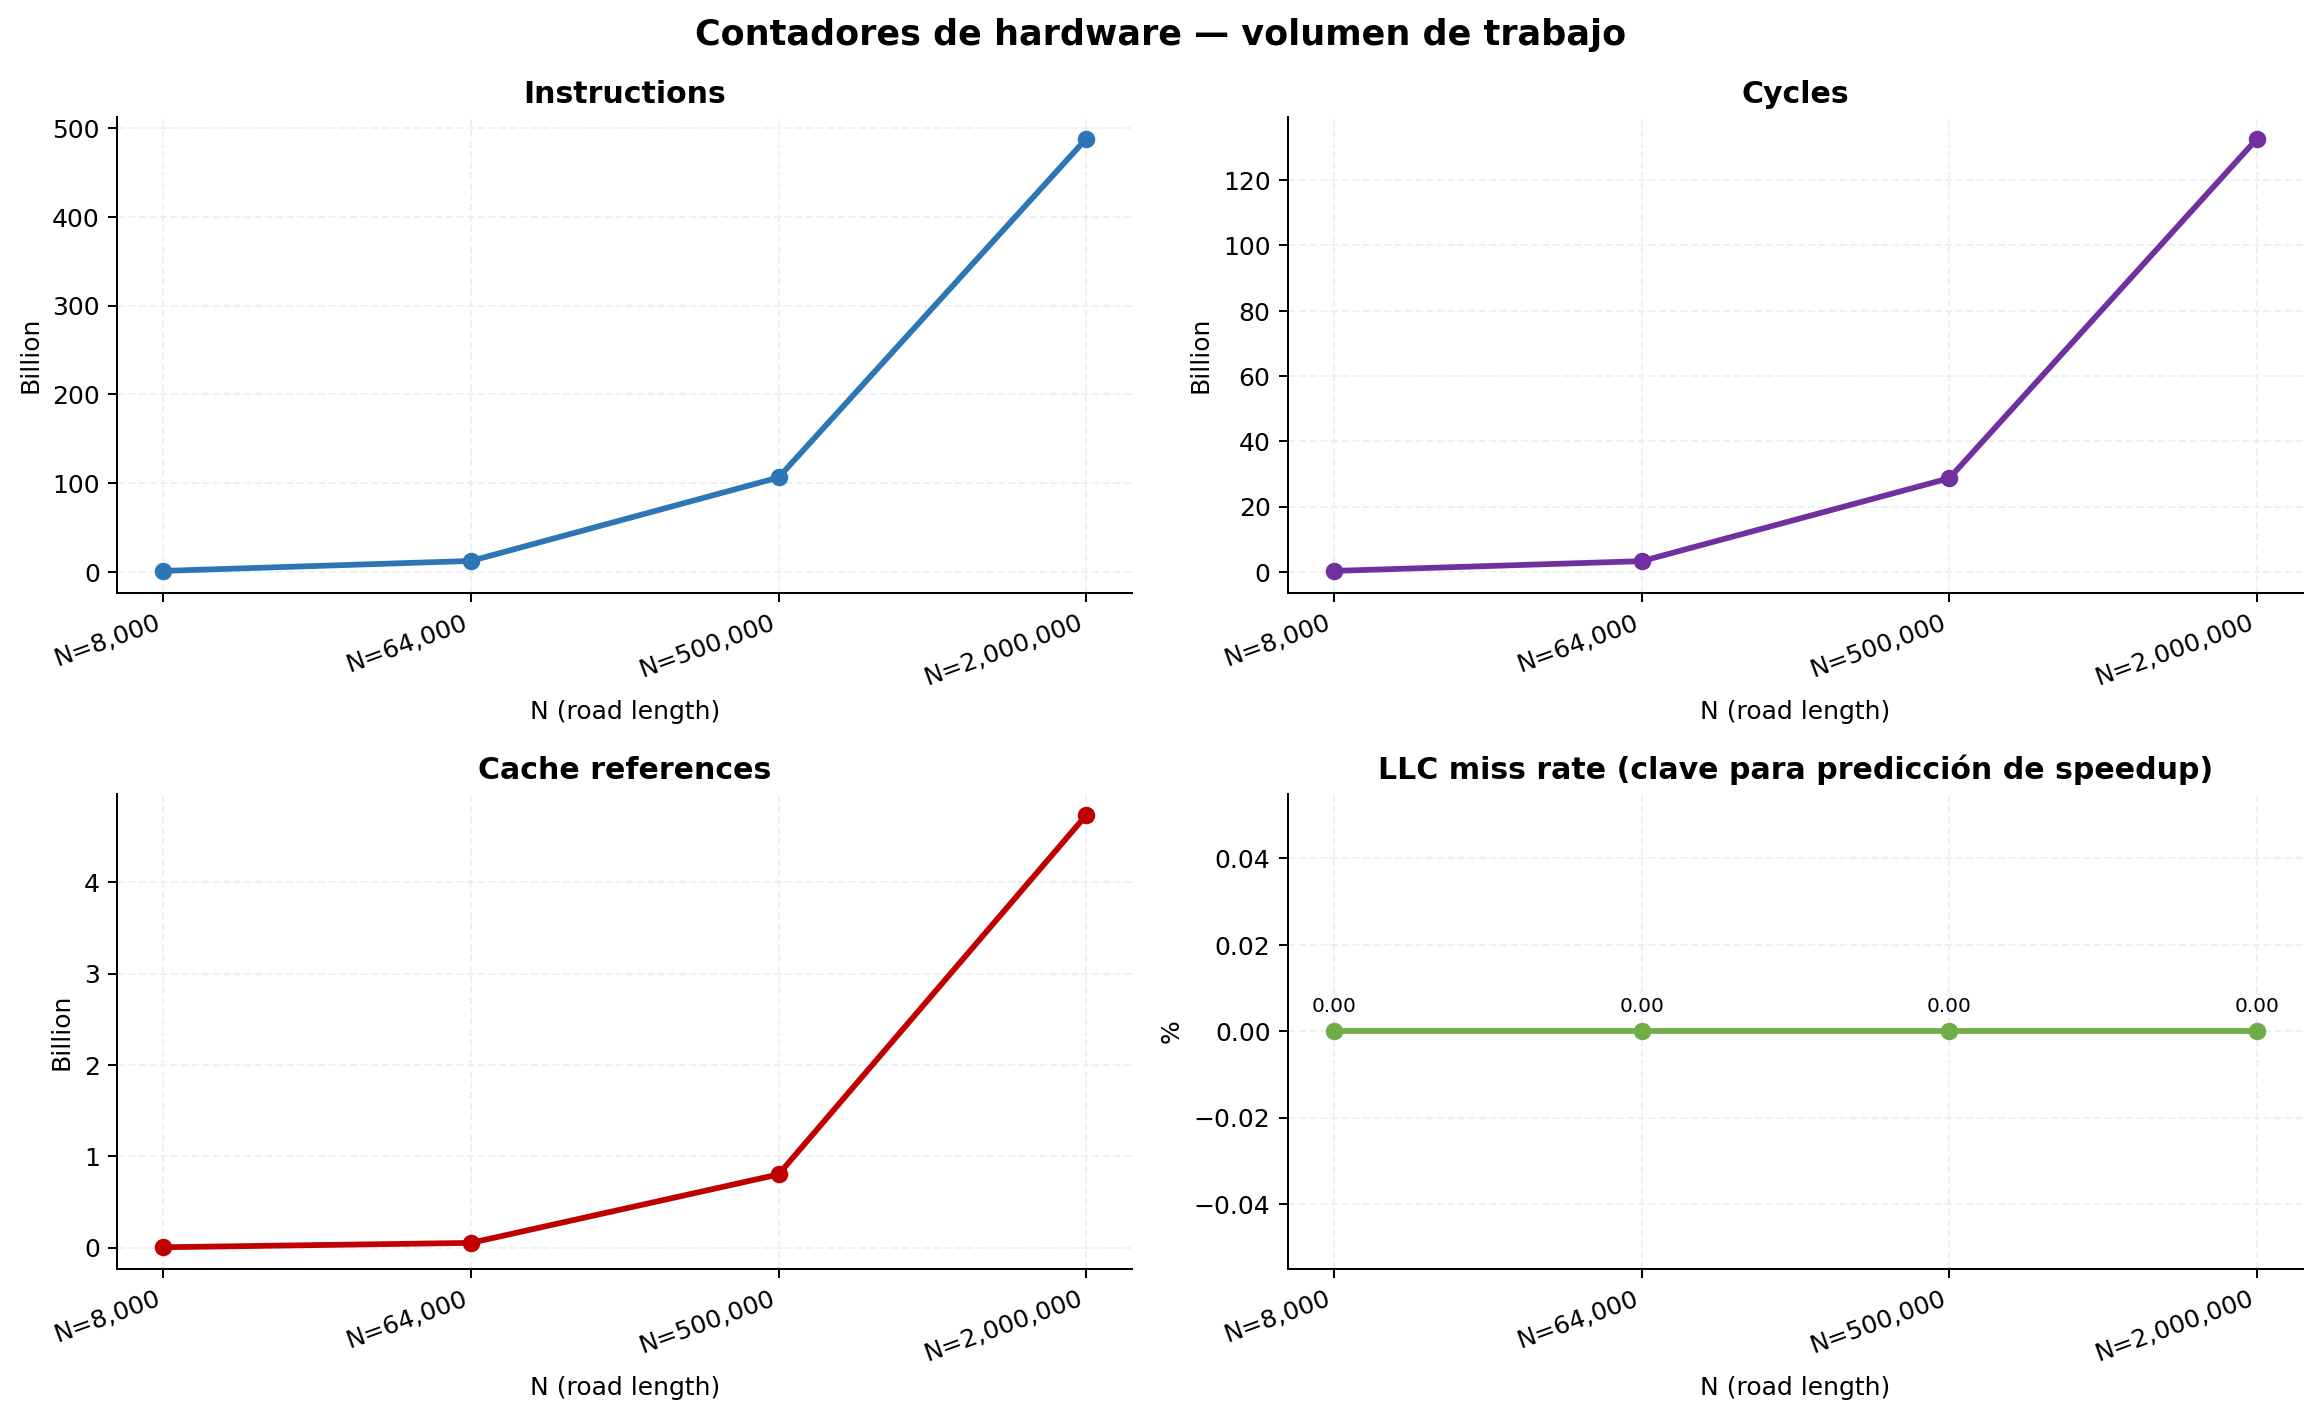
\includegraphics[width=1\textwidth]{images/profiling/04_counter_trends.png}
   \caption{Contadores de hardware}
   \label{fig:cache_summary}
\end{figure}

La tasa de fallos en L1 se sitúa en torno al 1.33--1.34\% de forma uniforme,
muy por debajo del 29.74\% observado en la multiplicación de matrices para
$N = 1024$ con patrón de acceso columnar.
La tasa de fallos de LLC es exactamente 0.00\% en todos los tamaños medidos,
incluyendo $N = 2000000$, cuyo working set teórico es $2 \times 2000000 \times 4
\approx 16$\,MB y supera la capacidad típica de L3.
Este resultado aparentemente contradictorio se explica por el prefetcher de hardware:
el acceso estrictamente secuencial al array de la carretera permite al prefetcher
cargar líneas de caché con suficiente anticipación como para que los accesos sean
atendidos sin registrar un fallo en LLC, aunque el dato haya sido traído desde DRAM.
El cuello de botella para $N$ grandes no es por tanto la latencia de caché sino el
ancho de banda del bus de memoria, que no queda directamente expuesto por los
contadores de LLC miss.

\begin{figure}[H]
   \centering
   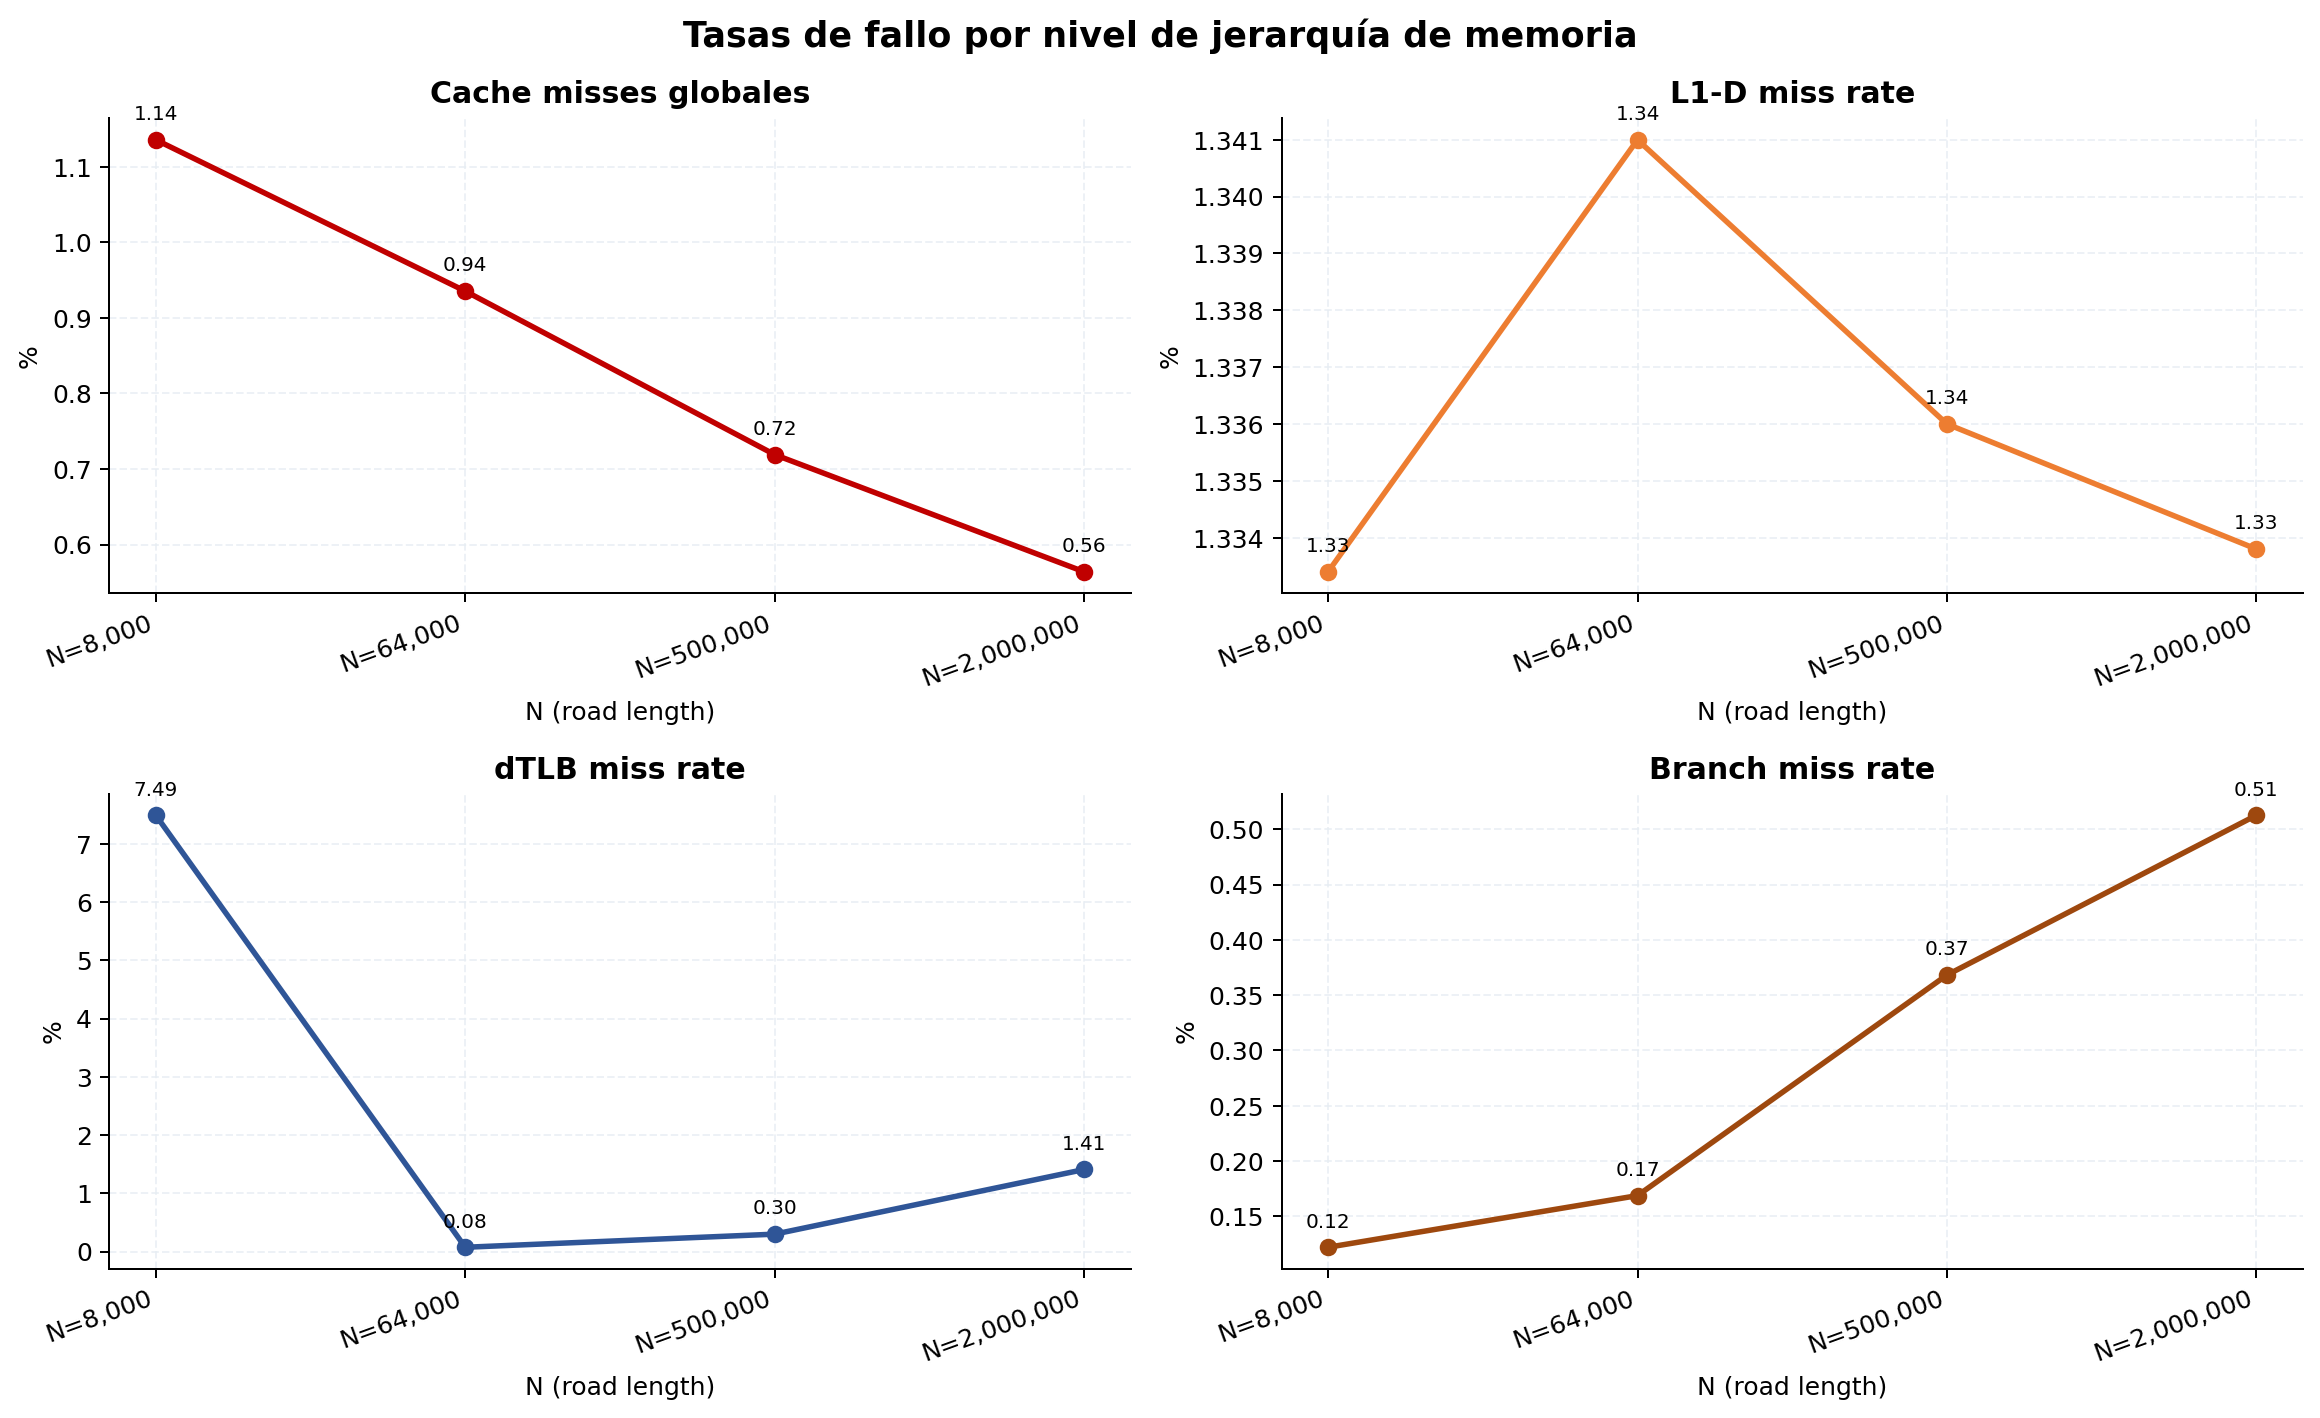
\includegraphics[width=1\textwidth]{images/profiling/03_miss_rates.png}
   \caption{Tasas de fallo de caché y TLB}
   \label{fig:cache_trends}
\end{figure}

Los fallos del predictor de ramas se mantienen por debajo del 0.52\% en todos
los casos, lo que es consistente con el flujo de control regular del bucle de
actualización.
El único contador con variabilidad notable entre tamaños es dTLB miss: el valor
elevado de 7.49\% para $N = 8000$ y su caída a 0.08\% para $N = 64000$ sugieren
que para la carretera más corta el acceso a las celdas mediante índice modular
genera un patrón de acceso a páginas virtuales que el TLB aún no tiene precargado
al inicio de la medición; al crecer $N$ las páginas se reutilizan con mayor
frecuencia y la presión sobre el TLB disminuye.


\subsubsection{Uso de memoria dinámica}

El análisis con Valgrind Massif muestra que el consumo de heap escala linealmente
con $N$, pasando de 0.061\,MB para $N = 8000$ hasta 3.815\,MB para $N = 500000$.
Este comportamiento coincide con el modelo teórico $M_{\text{teórico}} = 2 \cdot
N \cdot 4 / 1024^2$\,MB derivado de los dos arrays de enteros de tamaño $N$
reservados dinámicamente: la relación entre el valor medido y el teórico es del
99.94\% para $N = 8000$ y $N = 64000$, y del 100.01\% para $N = 500000$.
La fracción de bytes útiles respecto al total medido supera el 99.95\% en todos
los tamaños, lo que confirma que el gestor de memoria del sistema no introduce
overhead de fragmentación ni metadata anómala y que el consumo observado se explica
íntegramente por las reservas explícitas del programa.
Para $N = 2000000$ el valor teórico esperado es de aproximadamente 15.26\,MB,
pero Massif no pudo ejecutarse por superar el límite $N_{\max} = 500000$
establecido en el script.